%2025 - 4a
{}%
{\bf Chapitre 3 : Espace vectoriel tangent (suite)}

%{Vitesse d'une courbe en un point}%(rappel)
\subsection{rappels}
Une variété topologique de dimension n un ensemble de point munie d'une topologie et d'un atlas : (M, $\mc{O}$, $\mc{A}$).
Un atlas est un ensemble de cartes, une carte est une application homéomorphe d'un ouvert autour d'un point dans  $\mb{R}^\mt{n}$ :
\[
\mc{A} = \{ (\mc{U}, x) : \mc{U} \to \mb{R}^\mt{n}
\}
\]
Si l'atlas est restreint aux cartes qui peuvent être reliées par des transformations infiniment dérivables, on a une variété différentielle : (M, $\mc{O}$, $\mc{A}_\infty$).

 = localement (autour de chaque point), la variété est isomorphe à $\mb{R}^\mt{n}$ : $\mc{A}$ est un ensemble de cartes, les cartes étant des applications homéomorphe d'un ouvert autour de chaque point dans $\mb{R}^\mt{n}$ qui permet de donner des coordonnées aux points

\begin{minipage}[c]{.5\linewidth}
\[
\begin{array}{ l c l l }
 \gamma : & \mb{R} & \to & M \\ 
  & \lambda & \mapsto & \gamma(\lambda) \\
\end{array}
\]
\end{minipage}
\hfill
\begin{minipage}[c]{.5\linewidth}
\[
\begin{array}{ l c l l }
 {v}_{\gamma,p} : & \mc{C}^\infty(\mt{M}) & \to & \mb{R} \\ 
  & \mt{f} & \mapsto & {v}_{\gamma,p}(\mt{f})=(\mt{f}\circ\gamma)'|_{\lambda_0} \\
\end{array}
\]
\end{minipage}


\[
\gamma(\lambda_0)=p\in M
\]


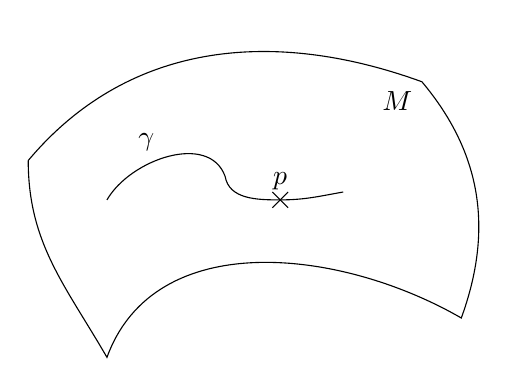
\begin{tikzpicture}
\draw(-3, 1) to[out=50, in=160] (2,2) node[below left]{$M$}
to[out=-50, in=70] (2.5,-1)
to[out=150, in=70] (-2,-1.5)
to[out=120, in=-90] (-3, 1); % Espace
%
\draw(-1.5,1) node[above]{$\gamma 	$};
\draw(-2,0.5) to[out=60, in=110] (-0.5,0.8)
to[out=-80, in=180]  (0.2,0.5) node[above]{$p$}
to[out=0, in=190] (1,0.6); % Courbe
%
\draw(0.1,0.6) -- (0.3,0.4);
\draw(0.1,0.4) -- (0.3,0.6);
\end{tikzpicture}
%{"Reparamétrage" d'une courbe}%
%{Espace vectoriel tangent, TpM : addition de deux vitesses et multiplication par un scalaire}%
%{Courbes coordonnées (d'une carte donnée) et vitesses associées}%
%{Base de TpM associée à une carte donnée}%
%{Notation importante : "dérivée partielle d'une fonction", représentée dans une carte}%
